% Evidence-bounded figure snippets for the ContextStore research draft.
% Paths are relative to docs/paper when the manuscript is converted to LaTeX.

\begin{figure*}[t]
  \centering
  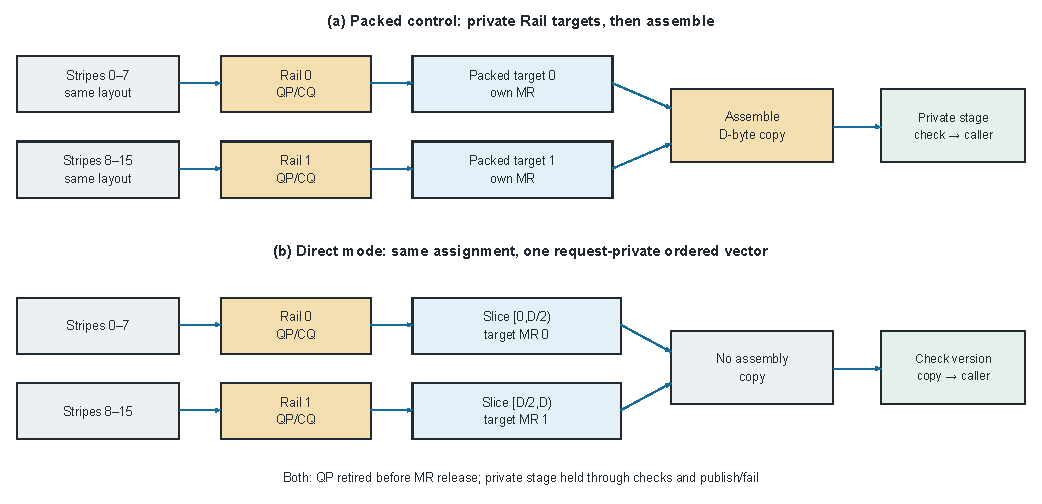
\includegraphics[width=0.96\textwidth]{figures/direct-vs-packed-2026-10-09-v1/contextstore-direct-vs-packed_en.pdf}
  \caption{Packed and direct private staging under the same equal-weight, 16-stripe example. Both Rails keep independent QP/CQ/MR lifetimes and both modes publish to the caller only after validation. Direct mode receives into disjoint slices of one private ordered vector, removing the packed-to-ordered assembly pass while retaining the final caller copy. This is a mechanism schematic, not a performance result.}
  \label{fig:direct-staging-mechanism}
\end{figure*}

\begin{figure*}[t]
  \centering
  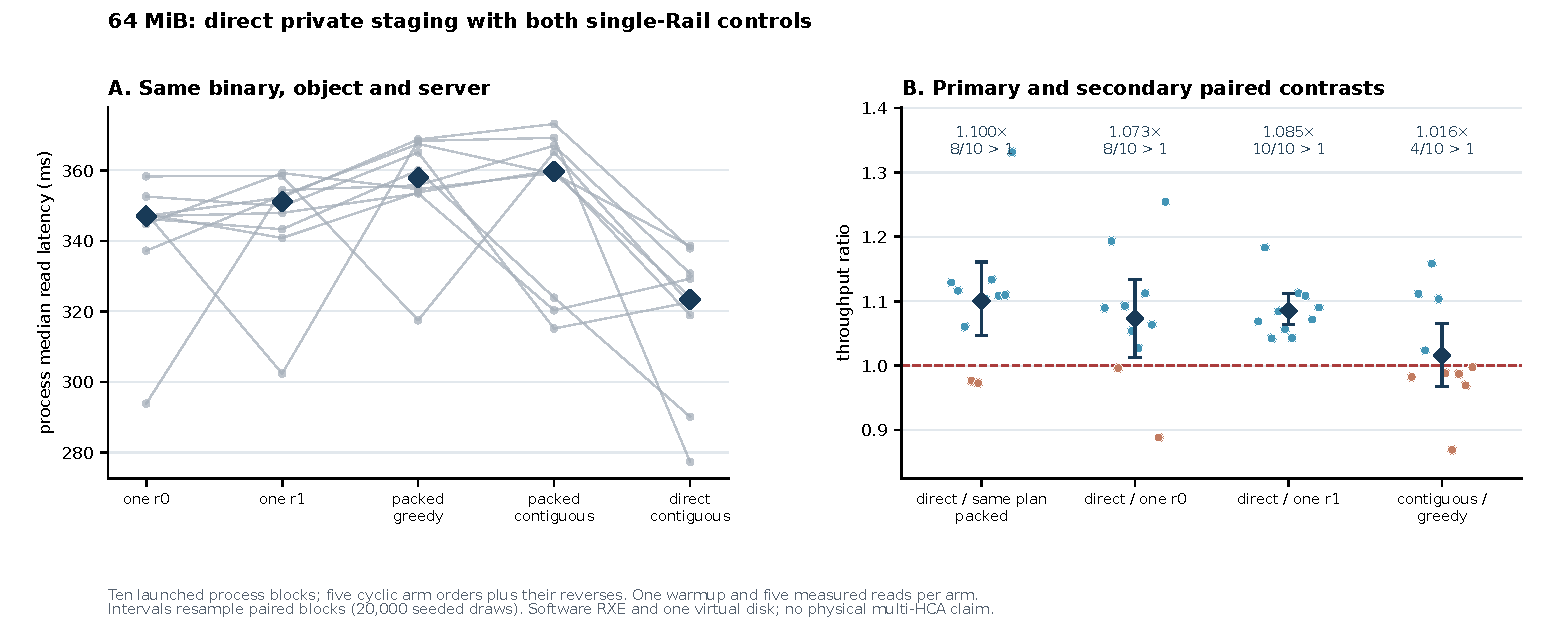
\includegraphics[width=0.96\textwidth]{figures/rail-five-arm-final-64-2026-10-09.pdf}
  \caption{64 MiB software-RXE five-arm experiment: ten balanced launched-process blocks, one warmup and five measured complete reads per arm. The predeclared direct/same-scheduler packed throughput ratio is 1.100$\times$ (95\% block-bootstrap interval 1.048--1.161$\times$). Both one-Rail paths and the original greedy scheduler are shown; the figure does not establish physical multi-HCA aggregation.}
  \label{fig:rxe-five-arm-64}
\end{figure*}

\begin{figure*}[t]
  \centering
  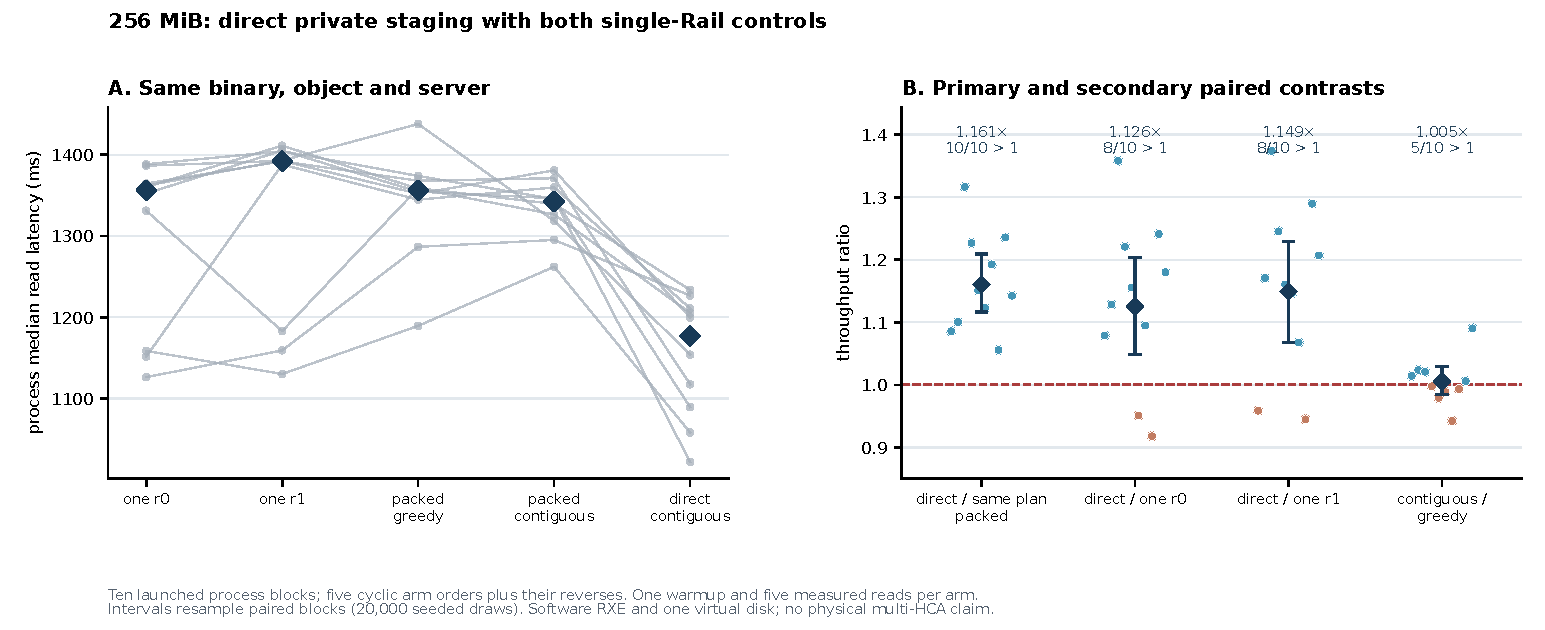
\includegraphics[width=0.96\textwidth]{figures/rail-five-arm-final-256-2026-10-09.pdf}
  \caption{256 MiB software-RXE five-arm experiment with the same block/order protocol. The direct/same-scheduler packed throughput ratio is 1.161$\times$ (95\% block-bootstrap interval 1.117--1.209$\times$). This object exceeds the server's 128 MiB RDMA slab and uses the registered-buffer fallback; trends across the two object sizes are therefore not an isolated size effect.}
  \label{fig:rxe-five-arm-256}
\end{figure*}

\begin{figure*}[t]
  \centering
  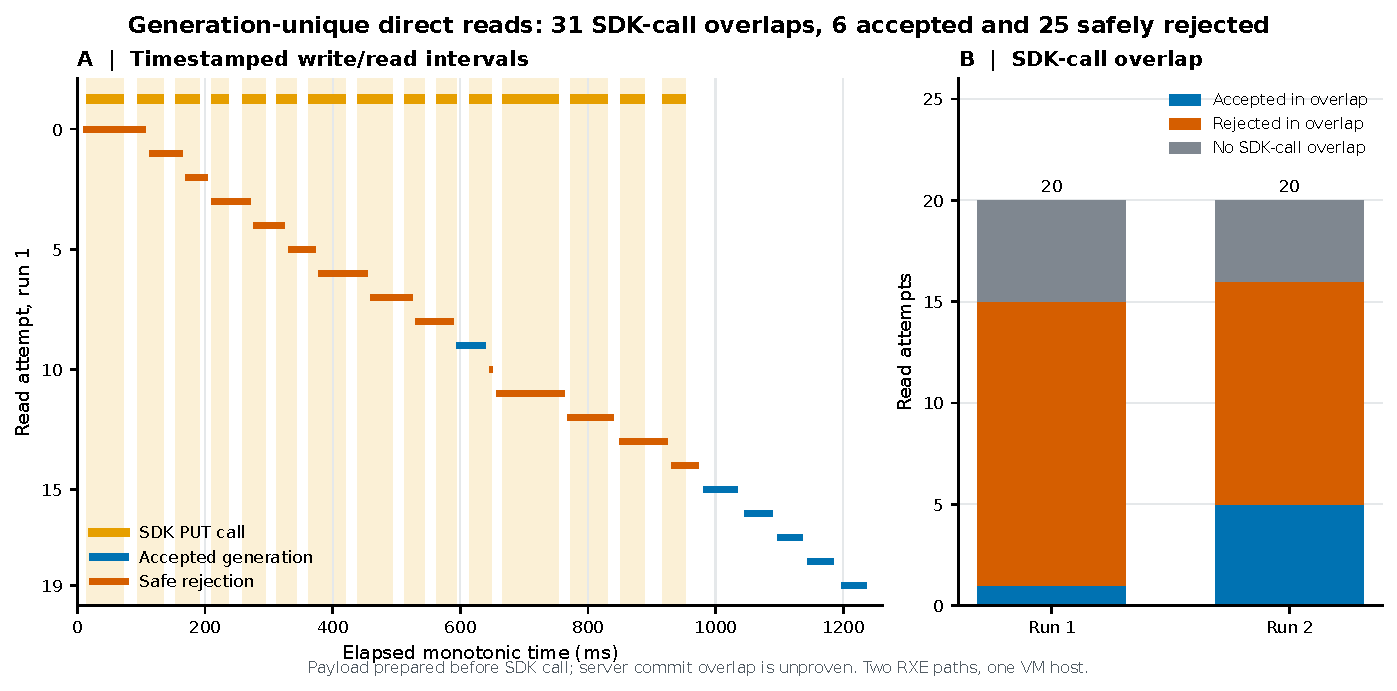
\includegraphics[width=0.96\textwidth]{figures/unique-generation-sdk-call-race-2026-10-09.pdf}
  \caption{Generation-unique direct two-Rail reads during concurrent SDK PUT calls in two isolated RXE guests. Payload allocation and segmentation finish before each write start timestamp. Panel A plots SDK call start-to-response windows and every read interval in one run; blue reads returned a byte-for-byte complete value matching the SDK-accepted Generation, and orange reads safely rejected. Panel B counts both runs: 31 of 40 attempts intersected an SDK call, six accepted and 25 rejected, with nine non-intersecting attempts shown separately. Server commit overlap remains unknown. These are observed software-Verbs schedules, not a proof of all interleavings or real-provider fault behavior.}
  \label{fig:unique-generation-sdk-call-overlap}
\end{figure*}
